\section{Analisi del problema e Soluzioni}
In questa sezione verrà descritto il problema affrontato, le soluzioni scelte ed i rispettivi
risultati ottenuti.

\paragraph{Problema affrontato}
Il problema affrontato chiedeva di trovare pattern, anomalie e/o inferire sui dataset forniti, 
per ottenere, come risultato, informazioni su di essi mediante l'utilizzo di tecniche 
dell'analisi di serie temporali.

Per questioni di tempo il problema è stato ridotto all'analisi dei giunti del piede, più in particolare,
il tirocinio, è stato basato, sulla ricerca di uno o più metodi necessari a trovare la lunghezza di un passo
(stride) con successiva analisi dei risultati.



\paragraph{Risultati aspettati}
\begin{sloppypar}
Come risultati aspettati è stata presa in considerazione l'eventualità della non riuscita dell'obbiettivo finale,
quindi l'impossibilità di trovare, tramite le tecniche dell'analisi di serie temporali, una possibile soluzione
al problema.
\end{sloppypar}

In caso positivo, quindi di una possibile soluzione al problema posto, i risultati aspettati potrebbero essere:
\begin{itemize}
    \setlength\itemsep{-0.5em}
    \item Capacità da parte del metodo sviluppato di rilevare la durata del passo.
    \item Capacità da parte del metodo sviluppato di rilevare incorrettamente la durata del passo.
    \item Impossibilità da parte del metodo sviluppato di rilevare un passo.
\end{itemize}


\subsection{Prima soluzione}
In questa sezione verrà mostrata la prima soluzione al problema posto, nello specifico verrà
spiegata in breve l'idea generale, l'implementazione di alcuni dei metodi utilizzati, l'analisi dei
risultati, l'analisi della complessità ed infine le conclusioni.


\subsubsection{Idea generale}
L'idea generale, fulcro di questa soluzione, ruota intorno all'analisi della funzione di autocorrelazione.
Quest'ultima viene utilizzata per riconoscere pattern o una sorta di correlazione tra i dati non
visibile direttamente.

\subsubsection{Implementazione}
Mediante l'ausilio del test di Dickey-Fuller ed il calcolo della prima differenza è stato possibile
rendere le serie stazionarie, preparandole così alla successiva analisi di autocorrelazione.
\\
\paragraph*{Snippet} (\textit{Prima differenza})
\begin{minted}{python3}
    def compute_first_diff(series: list | np.ndarray):
        """ Calcola la prima differenza
        """
        
        if not isinstance(series, np.ndarray):
            series = np.array(series)

        return series[1:] - series[:len(series)-1]
\end{minted}

\paragraph*{Snippet} (\textit{Metodo per rendere la serie stazionaria})
\begin{minted}{python3}
    def make_stationary(series, max_steps = 30):
        """ Rende la serie stazionaria mediante il calcolo
            della prima differenza
        """
        step = 0   # numero di step
        s_copy = series.copy()  # copia della serie
        
        # fino a quando il test ritornca che la serie
        # non è stazionaria oppure sono stati superati
        # il massimo di step
        while(sts.adfuller(series)[1] > 0.05 
            and step < max_steps):
            
            # calcola la prima differenza
            serie = compute_first_diff(series)
            step += 1

        # se max_step è superato, non si è riusciti
        # a rendere la serie stazionaria
        if step > 30:
            series = s_copy

        return series
\end{minted}

\begin{sloppypar}
Avendo reso ogni serie stazionaria guardiamo alcuni dei grafici relativi all'autocorrelazione
di serie appartenenti a dataset dei soggetti $6$ ed $8$.
\end{sloppypar}

\begin{figure}[H]
    \centering
    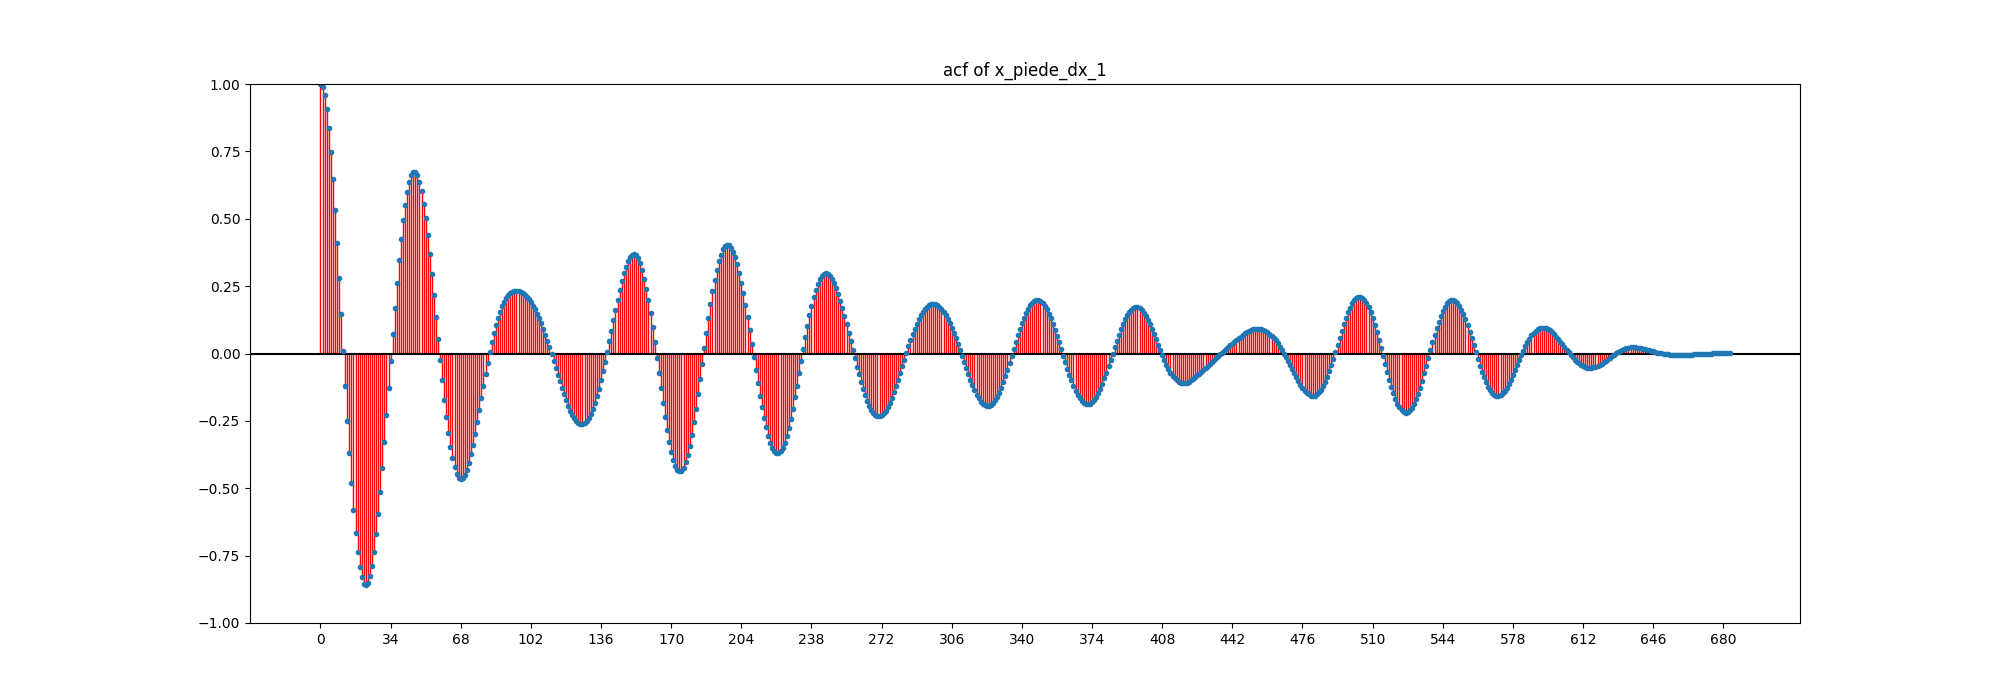
\includegraphics[width=\linewidth,keepaspectratio]{P006_x_piede_dx_1_acf.png}
    \caption{Soggetto $6$ autocorrelazione x piede destro posizione 1.}
    \label{fig:P006_x_piede_dx_1_acf}
\end{figure}

\begin{figure}[H]
    \centering
    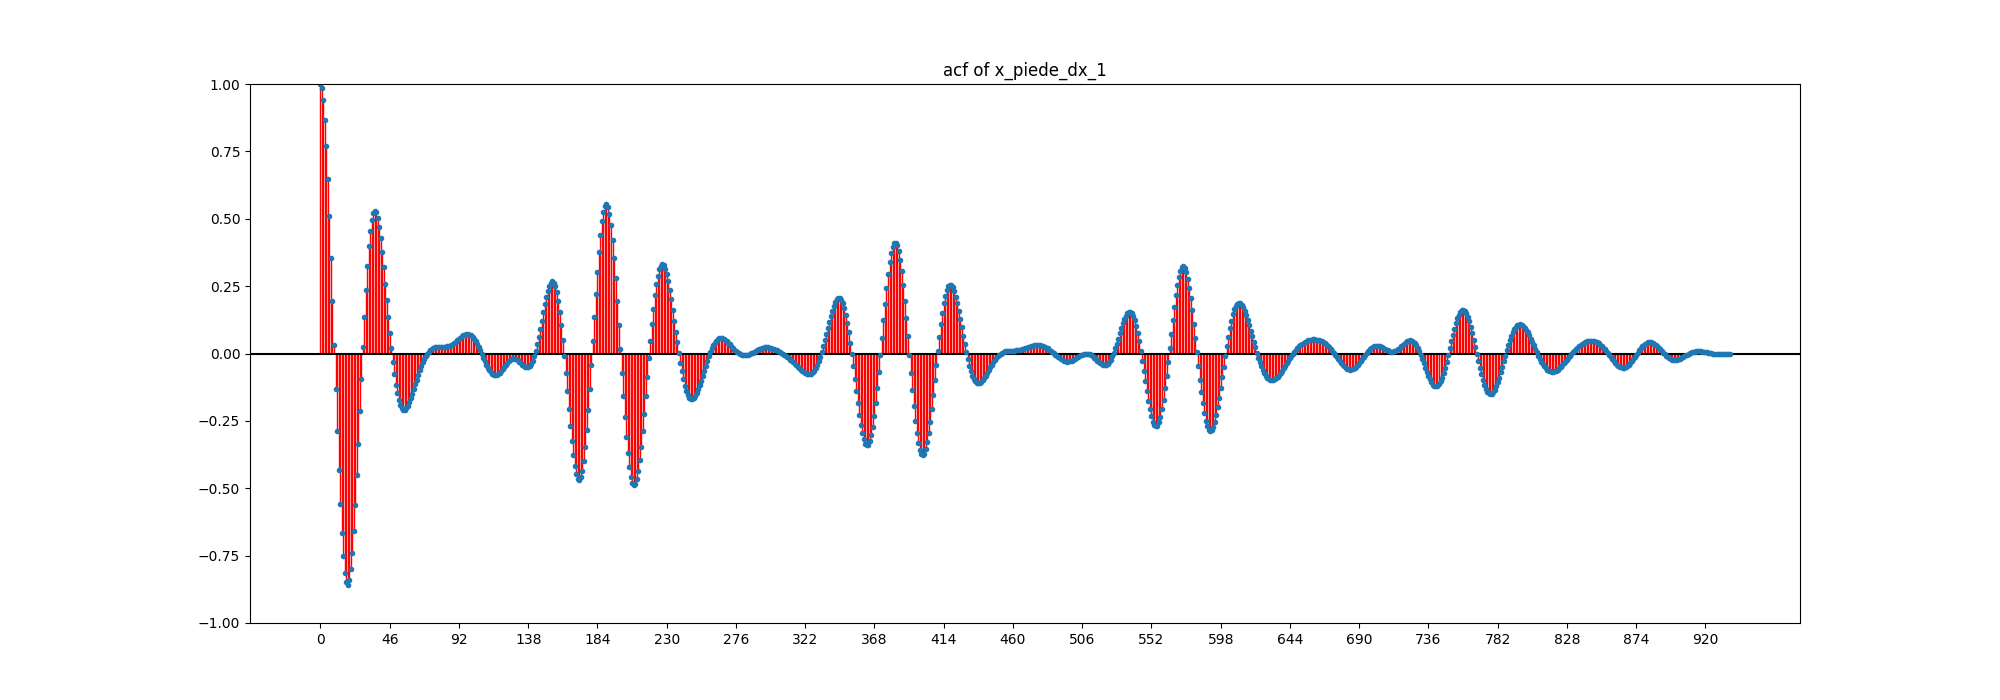
\includegraphics[width=\linewidth,keepaspectratio]{P008_x_piede_dx_1_acf.png}
    \caption{Soggetto $8$ autocorrelazione x piede destro posizione 1.}
    \label{fig:P008_x_piede_dx_1_acf}
\end{figure}

Da come si può notare dai grafici in figura~\ref{fig:P006_x_piede_dx_1_acf} e~\ref{fig:P008_x_piede_dx_1_acf}
l'autocorrelazione sembra riconoscere la durata di un passo in corrispondenza dei massimi locali.
\begin{sloppypar}
Utilizzando la funzione \texttt{argrelextrema} del modulo \texttt{statsmodels.tsa.stattools}
all'output della funzione di autocorrelazione è stato possibile recuperare gli argomenti (indici della lista) dei massimi locali.
Per esempio se prendiamo in considerazione il grafico~\ref{fig:P006_x_piede_dx_1_acf} gli argomenti
dei massimi locali sono
\end{sloppypar}
\[ [45, 95, 152, 197, 245, 297, 347, 395, 454, 504, 549, 592, 636, 678] \]
dove ogni argomento fa riferimento all'istante di tempo $t$, quindi al frame, in cui uno stride si ripete.

Questo ovviamente succede in linea teorica, non sempre è detto che il grafico dell'autocorrelazione
riesca ad ottenere con precisione quest'informazione, soprattutto se i dati non sono filtrati correttamente.

Continuado con l'implementazione del metodo, calcolando la distanza tra un argomento e l'altro troveremo
la durata di quel determinato passo. Prendendo sempre in considerazione la lista di agromenti sopra
e calcolandone la prima differenza otterremo
\[[50, 57, 45, 48, 52, 50, 48, 59, 50, 45, 43, 44, 42]\]
dove ogni elemento rappresenta la durata di un singolo stride.

Se calcoliamo la media otterremo la durata media di uno stride, che per la lista sopra sarà di 
$48.69\texttt{frame}$ cioè $1.623\texttt{secondi}$.


\paragraph{Snippet} (\textit{Metodo per il calcolo dello stride})
\begin{minted}{python3}
    def stride(serie: list | np.ndarray):
        """ Calcola la durata di uno stride
            assumendo che la serie sia stazionaria    
        """

        # redi la serie un array numpy
        if not isinstance(serie, np.ndarray):
            serie = np.array(serie)
        
        # funzione di autocorrelazione
        acf = funzione_autocorrelazione(serie)

        # prende gli argomenti massimi locali della acf
        arg_max_locali = argrelextrema(acf, np.greater)[0]

        # differenza tra gli argomenti massimi locali
        arg_max_locali_diff = compute_first_diff(arg_max_locali)

        # calcola durata media di uno stride
        media_stride = arg_max_locali_diff.mean()

        if not isinstance(serie, np.ndarray):
            arg_max_locali_diff = arg_max_locali_diff.tolist()

        return arg_max_locali_diff, media_stride

\end{minted}


Questa serie di metodi è stata successivamente applicata ad ogni dataset ottenendo così la durata
media di uno stride per ogni posizione del piede destro e sinistro. Per fare ciò è stato creato
un ``mini'' programma che esegue automaticamente queste istruzioni ad ogni serie.

\subsubsection{Analisi di complessità}
\begin{sloppypar}
Assumendo che la serie fornita sia già stazionaria la complessità di questo algoritmo 
deriva pricipalmente dalla complessità della funzione  \texttt{funzione\_autocorrelazione} e dalla complessità
della funzione \texttt{shift} utilizzata dalla funzione di autocorrelazione.
\end{sloppypar}

Se consideriamo $n$ come la lunghezza della serie, la funzione di autocorrelazione cicla $n$ volte
mentre la funzione di shift cicla $1,2,3,\dots,(n-2),(n-1),n$ volte quindi otterremo
una complessità temporale $O(n\log{n})$.

La complessità spaziale dell'algoritmo è $O(n)$.


\subsubsection{Analisi dei risultati e Conclusioni}
Per seplicità, i risultati verranno analizzati considerano un passo completo, cioè la somma degli stride
del piede destro e sinistro. Per fare chiarezza mostriamo un'immagine.
\begin{figure}[H]
    \centering
    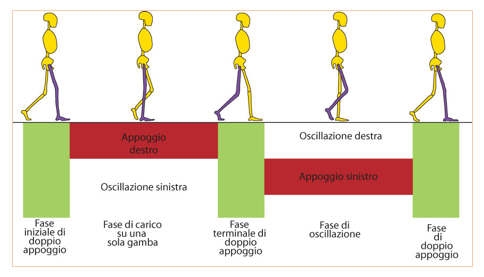
\includegraphics[width=0.8\linewidth,keepaspectratio]{passo_completo.png}
    \caption{Camminata di un soggetto~\cite{cf:passo_completo}.}
    \label{fig:passo_completo}
\end{figure}
Considerando la figura~\ref*{fig:passo_completo} stiamo valutando il periodo (durata) che parte dalla prima striscia
verde fino all'ultima striscia verde, quindi dall'inizio di una fase iniziale di doppio appoggio fino all'inzio
di un'altra fase iniziale di doppio appoggio.

\begin{sloppypar}
Detto ciò, compariamo ora la durata media dei passi completi dei soggetti sani e patologici. 

Si è trovato che la durata media di un passo completo con camminata normale è di rispettivamente $68,84 \ \texttt{frame}$
($2,294 \ \texttt{secondi}$) per i soggetti sani e di 
$81,71 \ \texttt{frame}$ ($2,723 \ \texttt{secondi}$) per i soggetti patologici.
I soggetti patologici, con camminata normale, hanno quindi una durata di passo completo maggiore del 
$19,84\%$ rispetto alla durata di un passo completo, con camminata normale, dei soggetti sani.
\end{sloppypar}

Applicando lo stesso ragionamento alle camminata tacco-punta e punta si è riscontrato che 
i soggetti patologici, con camminata tacco-punta, hanno una durata di passo completo maggiore del 
$8.28\%$ rispetto alla durata di un passo completo, con camminata tacco-punta, dei soggetti sani, 
mentre nella camminata punta si è riscontrata una durata maggiore del $43,04\%$.

I risultati ottenuti analizzando i dati delle camminate tacco-punta e punta non possono ritenersi affidabili
in quanto le percentuali e le medie sono state calcolate con troppe poche osservazioni.


\paragraph*{Premessa sui risultati}
I risultati sopra ottenuti non sono da prendere come riferimento in quanto essi sono ottenuti
mediante l'ausilio di un metodo non totalmente sicuro. Il metodo utilizzato è sperimentale e tantomeno 
fine allo scopo del tirocinio quindi potrebbe giungere a rislutati non corretti 
poichè la funzione di autocorrelazione potrebbe rilevare pattern e correlazioni diverse da quelle
aspettate ed anche perchè questa tecnica è stata applicata a seire filtrate in un certo modo.



\subsection{Seconda Soluzione}
In questa sezione verrà mostrata la seconda soluzione al problema posto, nello
specifico verrà spiegata in breve l’idea generale, l’implementazione di alcune parti relative all'algoritmo, 
l’analisi dei risultati, l’analisi della complessità ed infine
le conclusioni.

\subsubsection{Idea generale}
In questa soluzione al problema si è pensato di considerare la scoposizione delle serie nelle 
loro componenti quali trend, stagionalità e residui. Nello specifico l'idea è nata
pensado che possiamo considerare ad un passo (stride) di un soggetto come ad un evento periodico
che si ripete più o meno in ugual maniera nel tempo ad uno specifico periodo. Considerando quindi
la scoposizione nelle tre compnenti di una serie, la stagionaità ad un determinato periodo potrebbe
rappresentare l'informazione che stiamo cercando di ottenere. Questo avviene solamente il linea teorica
in quanto non è detto che il passo di un soggetto avvenga sempre ad intervalli precisi ma l'idea è che
ad un certo periodo la stagionalità raccolga la maggior parte dell'informazione cercata.

Essendo che questo processo si può provare attuare solamente guardando il grafico della stagionalità
si è pensato di automatizzarlo cercando un algoritmo che, data una serie temporare relativa ad un giunto,
esso dia come risultato un periodo
la cui stagionaità raccolga la maggior parte dell'informazione di un passo. Per fare ciò è stato 
necessario comparare due serie, o meglio detto, è stato necessario comparare la serie relativa 
ad un giunto divisa a metà considerando le due metà come serie separate. Successivamente
si è calcolata la stagionalità su più periodi per entrambe le serie. In linea teorica i periodi con
stagionalità simili sarebbero dovute essere i pattern che occorrono in entrambe le serie,
mentre le stagionalità ``diverse'' sarebbero dovute essere pattern che non rientrano 
in entrambe probabilmente dovuto ad altre motivazioni quali, ad esempio, del rumore ancora presente.





\subsubsection{Implementazione}
Per prima cosa è necessario dividere una serie relativa ad un giunto di un soggetto in due e decidere
su quali periodi calcolare la stagionalità.

Successivamente per ogni periodo si è calcolata la stagionalità delle due parti
calcolandone la differenza quindi l'errore tra le due stagionalità. Per calcolare la stagionalità
è stata utilizzata la funzione \texttt{seasonal\_decompose} del modulo \texttt{statsmodels.tsa.seasonal}
relativo al pacchetto \texttt{statsmodels}, mentre per il calcolo dell'errore
le due stagionalità sono state convertite nel dominio delle frequenze, utilizzando la trasformata
di Fourier, e calcolata la differenza di ampiezza tra frequenze. L'algoritmo è stato 
creato per poter accettare anche serie divise in più di due parti.

Vediamo ora come è stata implementata la funzione che esegue il calcolo dell'errore.

\paragraph*{Snippet} (\textit{Calcolo dell'errore tra stagionalità})
\begin{minted}{python3}
    def freq_error(season_1: list, season_2: list):

        # prendi la lunghezza minima 
        min_len = 0
        if len(season_1) < len(season_2):
            min_len = len(season_1)
        else:
            min_len = len(season_2)

        # calcolo della trasformata di 
        # Fourier tra stagionalità
        fft_season_1 = sft.fft(season_1, min_len)
        fft_season_2 = sft.fft(season_2, min_len)

        # calcolo del magnitudo per ogni trasformata
        fft_season_1_m = np.abs(fft_season_1) / len(season_1)
        fft_season_2_m = np.abs(fft_season_2) / len(season_2)

        # differenza tra frequenze
        fft_diff = []
        for idx in range(min_len//2):
            fft_diff.append(fft_season_1_m[idx] - fft_season_2_m[idx])
        
        # calcolo dell'errore quadratico medio
        return np.power(fft_diff, 2).mean() 
\end{minted}


Vediamo ora il metodo principale.
\paragraph*{Snippet} (\textit{Metodo per la soluzione al problema (2)})
\begin{minted}{python3}
    def soluzione_2(seriesList, periods):
        """ 
        seriesList = 
                lista che contiene la serie divisa in due parti
                quindi due liste

        periods = 
                lista di interi, è la lista che
                contiene i periodi su cui calcolare
                la stagionalità
        """
        # per ogni periodo
        errors = []
        for j, period in enumerate(periods):

            # non è possibile calcolare 
            # la stagionalità per il periodo 0
            if period == 0:
                raise Exception('stagionalità non calcolabile \
                    con periodo 0')

            # calcola l'errore le parti della serie
            aux_errors = []
            for idx, series in enumerate(seriesList):

                # stagionalità della prima parte
                season = seasonal_decompose(
                    series, period=period).seasonal

                
                for idx in range(idx+1, len(seriesList)):

                    # stagionalità della seconda parte 
                    # (e altre parti)
                    aux_season = seasonal_decompose(
                        seriesList[idx], period=period).seasonal
                    
                    # calcolo dell'errore tra stagionalità
                    aux_errors.append(
                        freq_error(season, aux_season)
                    )
            

            errors.append(np.mean(aux_errors))

        return np.min(errors), periods[np.argmin(errors)], errors
\end{minted}

Come possiamo vedere dall'implementazione come risultato otteniamo l'errore minimo, il periodo
associato all'errore minimo e la lista contenente, per ogni periodo, l'errore associato.

In una fase successiva è stata creata una funzione che permette di analizzare la lista relativa
agli errori per ogni periodo creando dei grafici che indicano i periodi ``salienti''. 
L'implementazione di quet'ultima non verrà data ma il concetto è che per periodi piccoli l'errore
è sempre il minimo e crescente e, dopo un certo periodo, l'errore inizia ad aumentare drasticamente
per poi diminuire successivamente dopo aver trovato una stagionalià nuovamente simile tra le due serie.
Per capire meglio consideriamo la lista degli errori tra $1$ e $30$, in questo range l'errore è crescente
per ogni periodo, dal periodo $31$ in poi l'errore aumenta drasticamente fino al periodo $80$ per poi diminuire
nuovamente ed ad un certo punto riaumentare. Questo è dovuto appunto al fatto che quando le stagionalità non si
``assomigliano'' l'errore sarà alto mentre per stagionalità simili l'errore è minimo o comunque molto basso.


\subsubsection{Analisi dei risultati}
Analizziamo ora qualche grafico cercando di capire meglio come rappresentare i risultati del metodo
spiegato nella sezione precedente.






\subsubsection{Analisi di complessità}
\subsubsection{Conclusioni}